
\chapter{How to write reusable apps}

\section{Your project and your reusable app}

The project structure is shown in Figure \ref{fig:project}
\begin{figure}[!ht]
  \centering
  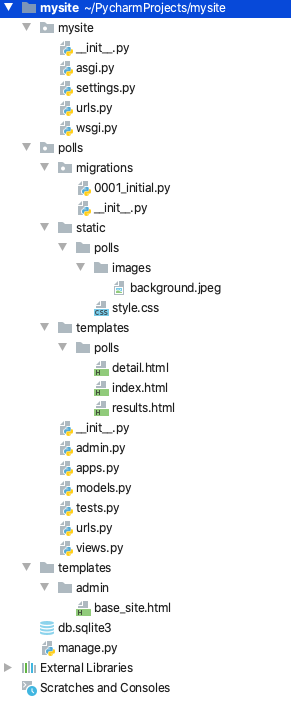
\includegraphics[height=\textheight]{project.png}
  \caption{Project}
  \label{fig:project}
\end{figure}


\section{Packaging your app}

Python packaging refers to preparing your app in a specific format that can be easily installed and used.
For a small app like polls, this process isn’t too difficult.


\begin{enumerate}
\item Create a parent directory for \keyword{polls}, outside of your Django project. Call this directory \keyword{django-polls}.
\item Move the \keyword{polls} directory into the django-polls directory.
\item Create a file \keyword{django-polls/README.rst} with the following contents:
  \begin{tcolorbox}
    \tiny{
\begin{verbatim}
=====
Polls
=====

Polls is a Django app to conduct Web-based polls. For each question,
visitors can choose between a fixed number of answers.

Detailed documentation is in the "docs" directory.

Quick start
-----------

1. Add "polls" to your INSTALLED_APPS setting like this::

    INSTALLED_APPS = [
        ...
        'polls',
    ]

2. Include the polls URLconf in your project urls.py like this::

    path('polls/', include('polls.urls')),

3. Run ``python manage.py migrate`` to create the polls models.

4. Start the development server and visit http://127.0.0.1:8000/admin/
   to create a poll (you'll need the Admin app enabled).

5. Visit http://127.0.0.1:8000/polls/ to participate in the poll.

\end{verbatim}
    }
    
  \end{tcolorbox}
  
\item Create a \keyword{django-polls/LICENSE} file.
\item Create \keyword{setup.cfg} and \keyword{setup.py} files which detail how to build and install the app.
  \begin{tcolorbox}
    django-polls/setup.cfg
    \begin{lstlisting}
      [metadata]
      name = django-polls
      version = 0.1
      description = A Django app to conduct Web-based polls.
      long_description = file: README.rst
      url = https://www.example.com/
      author = Your Name
      author_email = yourname@example.com
      license = BSD-3-Clause  # Example license
      classifiers =
      Environment :: Web Environment
      Framework :: Django
      Framework :: Django :: X.Y  # Replace "X.Y" as appropriate
      Intended Audience :: Developers
      License :: OSI Approved :: BSD License
      Operating System :: OS Independent
      Programming Language :: Python
      Programming Language :: Python :: 3
      Programming Language :: Python :: 3 :: Only
      Programming Language :: Python :: 3.6
      Programming Language :: Python :: 3.7
      Programming Language :: Python :: 3.8
      Topic :: Internet :: WWW/HTTP
      Topic :: Internet :: WWW/HTTP :: Dynamic Content

      [options]
      include_package_data = true
      packages = find:
    \end{lstlisting}
  \end{tcolorbox}

  \begin{tcolorbox}
    django-polls/setup.py
    \begin{lstlisting}
      from setuptools import setup

      setup()
    \end{lstlisting}
  \end{tcolorbox}
\item Only Python modules and packages are included in the package by default. To include additional files, we’ll need to create a \keyword{MANIFEST.in} file.
  \begin{tcolorbox}
    \begin{lstlisting}
      include LICENSE
      include README.rst
      recursive-include polls/static *
      recursive-include polls/templates *
    \end{lstlisting}
  \end{tcolorbox}
  
\item It’s optional, but recommended, to include detailed documentation with your app. Create an empty directory \keyword{django-polls/docs} for future documentation. Add an additional line to \keyword{django-polls/MANIFEST.in}
  \begin{lstlisting}
    recursive-include doc *
  \end{lstlisting}
  
\item Try building your package with \keyword{python setup.py sdist} (run from inside \keyword{django-polls}). This creates a directory called \keyword{dist} and builds your new package, \keyword{django-polls-0.1.tar.gz}.
\end{enumerate}


\section{Using your own package}

\begin{enumerate}
\item To install the package
  \lstset{language=Sh}
  \begin{lstlisting}
    python -m pip install --user django-polls/dist/django-polls-0.1.tar.gz
  \end{lstlisting}
\item With luck, your Django project should now work correctly again. Run the server again to confirm this.
\item To uninstall the package, use pip:
  \begin{lstlisting}
    python -m pip uninstall django-polls
  \end{lstlisting}
\end{enumerate}


